\documentclass[conference]{IEEEtran}
\IEEEoverridecommandlockouts
\usepackage{cite}
\usepackage{amsmath,amssymb,amsfonts}
\usepackage{algorithmic}
\usepackage{graphicx}
\usepackage{textcomp}
\usepackage{xcolor}
\usepackage{booktabs}
\usepackage{pgfplots}
\pgfplotsset{compat=1.18}
\def\BibTeX{{\rm B\kern-.05em{\sc i\kern-.025em b}\kern-.08em
    T\kern-.1667em\lower.7ex\hbox{E}\kern-.125emX}}
\begin{document}

\title{Steal or Wait? Evaluating Work-Stealing Scheduler Policies in a Native C HTTP Server}

\author{\IEEEauthorblockN{Hamid Riaz}
\IEEEauthorblockA{\textit{University of Engineering and Technology}}}

\maketitle

\begin{abstract}
This paper evaluates four thread-scheduling policies for a native C HTTP/1.1 file server built on epoll edge-triggered I/O and POSIX threads. The baseline dispatches connections via round-robin (RR) to mutex-protected FIFO queues. Three work-stealing (WS) policies---random steal (RS), longest-queue steal (LQS), and adaptive steal (AS)---use a Chase-Lev lock-free deque per worker to rebalance load dynamically. All policies are benchmarked with wrk at 1, 2, 4, and 8 threads serving small static files. RS achieves the highest throughput (10,528~req/s at 8 threads, a 3.51$\times$ improvement over RR) with consistently low tail latency (175~$\mu$s p99). LQS shows a unique advantage at 2 threads---the only policy to improve over its own 1-thread baseline---but degrades at higher counts as its O(p) scan cost grows. AS, which dynamically adapts its steal threshold via a p99 latency feedback loop, underperforms both simpler policies, exhibiting the worst p99 latency (524~$\mu$s) at 4--8 threads. An Amdahl analysis confirms that RR's single-threaded accept loop is the primary serial bottleneck. Due to hardware constraints, the load generator and server were co-located on the same machine; this depresses absolute throughput at higher thread counts but does not affect relative comparisons between policies.
\end{abstract}

\begin{IEEEkeywords}
work stealing, thread scheduling, HTTP server, epoll, Chase-Lev deque, load balancing
\end{IEEEkeywords}

\section{Introduction}

The C10K problem~\cite{b6} identified the challenge of scaling Internet servers to tens of thousands of concurrent connections, and modern multi-core hardware has only amplified the need for efficient parallel request dispatch. An HTTP server must accept connections, parse requests, read files, and send responses---all while minimizing latency and maximizing throughput. Heterogeneous workloads (varying file sizes, mixed static and dynamic requests) introduce load imbalance that naive dispatch strategies handle poorly~\cite{b7,b8}.

Round-robin (RR) dispatch, the simplest parallel approach, assigns each new connection to the next worker in a fixed rotation. While O(1) at dispatch time, RR is oblivious to the actual load on each worker. A worker that receives a large file transfer or a slow CGI request remains busy while others idle. The dispatch thread itself becomes a serial bottleneck as connection rates rise.

Work stealing~\cite{b1} provides a decentralized alternative: each worker maintains its own task queue, and idle workers steal tasks from busy peers. Originally developed for multithreaded computations in the Cilk system~\cite{b2}, work stealing has been adopted widely---in Java's Fork/Join framework~\cite{b20}, the Go scheduler, and Rust's Tokio runtime. The Chase-Lev lock-free deque~\cite{b3} makes practical work stealing efficient by allowing the owner to push and pop from one end without synchronization while thieves steal from the other end with a single compare-and-swap (CAS). Recent work has extended work stealing to interactive services with latency targets~\cite{b5} and formally verified the correctness of block-based variants~\cite{b4}.

Despite this body of work, no prior study compares random steal, longest-queue steal, and adaptive steal policies head-to-head in a native C HTTP server with rigorous per-policy scaling analysis. This paper fills that gap with the following contributions:

\begin{itemize}
\item A complete, open-source C HTTP/1.1 server using epoll edge-triggered I/O, \texttt{sendfile()} for zero-copy transfers, and a modular scheduler framework supporting four policies.
\item A quantitative comparison of RR, RS, LQS, and AS across 1, 2, 4, and 8 threads, measuring throughput, p99 latency, speedup, and weak-scaling efficiency.
\item An Amdahl's Law analysis quantifying the serial dispatch bottleneck in the RR baseline.
\item Steal-accounting data showing the overhead of each policy.
\end{itemize}

\section{Sequential Baseline}

The sequential server serves as the foundation for all parallel variants. It uses a single-threaded event loop based on epoll in edge-triggered (EPOLLET) mode.

\begin{algorithmic}
\STATE Create epoll instance $efd$
\STATE Bind and listen on TCP port 8080
\STATE Register listen socket with epoll (EPOLLIN $|$ EPOLLET)
\LOOP
    \STATE $nfds \gets$ \texttt{epoll\_wait($efd$, events, maxevents, -1)}
    \FOR{$i = 0$ \TO $nfds-1$}
        \IF{$events[i].data.fd$ is listen socket}
            \WHILE{true}
                \STATE $conn \gets$ \texttt{accept(fd, \ldots)}
                \IF{$conn < 0$} \STATE break \ENDIF
                \STATE Set $conn$ non-blocking
                \STATE Register $conn$ with epoll (EPOLLIN $|$ EPOLLET $|$ EPOLLONESHOT)
            \ENDWHILE
        \ELSE
            \STATE \texttt{read($fd$, buf, sizeof(buf))}
            \STATE Parse HTTP method, path, and headers
            \STATE \texttt{stat(path, \&st)} to get file metadata
            \STATE Open file: \texttt{open(path, O\_RDONLY)}
            \STATE \texttt{sendfile($fd$, file\_fd, \&offset, st.st\_size)}
            \STATE \texttt{close(file\_fd)}; \texttt{close($fd$)}
        \ENDIF
    \ENDFOR
\ENDLOOP
\end{algorithmic}

The pipeline for each request is: \texttt{accept $\rightarrow$ parse $\rightarrow$ stat $\rightarrow$ open $\rightarrow$ sendfile $\rightarrow$ close}. By using \texttt{sendfile()}, the server avoids copying file data through user space---a zero-copy transfer performed entirely in kernel space~\cite{b12}.

\textit{Time complexity:} Each request performs O(1) fixed work: one header parse, one \texttt{stat} call, and one \texttt{sendfile} syscall. The epoll event loop dispatches ready events in O(N) for N concurrent connections.

\textit{Space complexity:} O(N) for connection state structs (file descriptor, read buffer, parse state), plus one 4~KB read buffer per connection. The \texttt{sendfile} path requires no per-request heap allocation.

The sequential baseline achieves 12,102~req/s serving 4~KB files. This value serves as the 1-thread reference for all speedup calculations; work-stealing variants incur non-trivial initialization overhead (deque allocation, thread startup) even at 1 thread, so the RR@1T measurement provides a cleaner sequential reference point.

\section{Parallel Design}

\subsection{Pthreads --- Round-Robin (Baseline Parallel)}

In the RR parallel server, one main thread runs the epoll accept loop (\S2) and pushes accepted connections onto per-worker FIFO queues. Each of $p$ worker threads owns a mutex-protected queue and a condition variable for signaling.

\begin{algorithmic}
\STATE \textbf{Main thread (dispatch):}
\STATE $counter \gets 0$
\LOOP
    \STATE $conn \gets$ \texttt{accept(...)} (via epoll)
    \STATE $target \gets counter \ \%\ num\_workers$
    \STATE $counter \gets counter + 1$
    \STATE \texttt{pthread\_mutex\_lock(\&queues[$target$].lock)}
    \STATE \texttt{queue\_push(\&queues[$target$], conn)}
    \STATE \texttt{pthread\_mutex\_unlock(\&queues[$target$].lock)}
    \STATE \texttt{pthread\_cond\_signal(\&queues[$target$].cond)}
\ENDLOOP
\end{algorithmic}

\begin{algorithmic}
\STATE \textbf{Worker thread (all workers):}
\LOOP
    \STATE \texttt{pthread\_mutex\_lock(\&queue.lock)}
    \WHILE{queue is empty}
        \STATE \texttt{pthread\_cond\_wait(\&queue.cond, \&queue.lock)}
    \ENDWHILE
    \STATE $conn \gets$ \texttt{queue\_pop(\&queue)}
    \STATE \texttt{pthread\_mutex\_unlock(\&queue.lock)}
    \STATE Serve $conn$ (parse, sendfile, close)
\ENDLOOP
\end{algorithmic}

This design is straightforward: the dispatch is O(1), each worker handles its own requests independently, and there is no shared state between workers during request processing. However, the mutex-protected queue access serializes every enqueue and dequeue operation.

\subsection{Pthreads --- Work-Stealing Variants (RS, LQS, AS)}

All three work-stealing variants replace the per-worker FIFO queues with Chase-Lev lock-free double-ended deques~\cite{b3}. Each deque supports three operations:

\begin{itemize}
    \item \texttt{push\_bottom(task)}: the owner thread appends a task to the bottom of its deque. No synchronization needed; single-writer guarantee.
    \item \texttt{pop\_bottom()}: the owner removes and returns the most recently added task from the bottom. Again no synchronization.
    \item \texttt{pop\_top()}: a thief thread attempts to remove and return the oldest task from the top of a victim's deque. Implemented with a single CAS on the top index, with a version counter to resolve the ABA problem.
\end{itemize}

The generic worker loop for all WS variants is:

\begin{algorithmic}
\STATE \textbf{Worker thread (WS variants):}
\LOOP
    \IF{\texttt{pop\_bottom(deque)} returns a task}
        \STATE Serve the task (parse, sendfile, close)
    \ELSE
        \STATE $victim \gets$ \texttt{choose\_victim()}
        \IF{\texttt{pop\_top(deque[$victim$])} returns a task}
            \STATE Increment steal-success counter
            \STATE Serve the task
        \ELSE
            \STATE Increment steal-attempt counter (failed)
        \ENDIF
    \ENDIF
\ENDLOOP
\end{algorithmic}

The three policies differ only in \texttt{choose\_victim()}:

\textbf{Random Steal (RS):} The thief selects a victim uniformly at random: $victim = rand()\ \%\ num\_workers$, skipping itself. This is the classic Cilk policy~\cite{b1}. It is O(1) per steal attempt and requires no global knowledge.

\textbf{Longest-Queue Steal (LQS):} The thief scans all worker deques, reading each deque's size with an atomic load, and selects the deque with the maximum length. This is O(p) per steal attempt. When $p=2$, the scan costs only one comparison---effectively free---while providing perfect load balancing between two queues.

\textbf{Adaptive Steal (AS):} Each worker maintains an exponential moving average (EMA) of the p99 request latency:
\begin{equation}
L_{t+1} = \alpha \cdot L_{measured} + (1-\alpha) \cdot L_t
\label{eq:ema}
\end{equation}
where $\alpha = 0.125$. The worker compares $L_t$ against a target latency $T_{target}$ (set to 200~$\mu$s). When $L_t > T_{target}$, the worker reduces its steal threshold (steals after fewer failed local pops); when $L_t < T_{target}$, it waits longer before stealing. The steal threshold $\tau$ is updated as:
\begin{equation}
\tau_{t+1} = \tau_t + \beta \cdot (T_{target} - L_t)
\label{eq:tau}
\end{equation}
with $\beta = 0.01$. The feedback loop aims to reduce idle spinning under low load while increasing steal aggressiveness under high load.

All three variants use per-thread atomic counters for steal attempts, steal successes, and queue depth. There is no shared mutable state between workers during normal task execution.

\section{Experimental Setup}

Experiments were conducted on a single machine with the following configuration:

\begin{itemize}
    \item \textbf{CPU:} Intel(R) Core(TM) i5-8350U CPU @ 1.70{}GHz (max 3.60{}GHz), 4 physical cores (8 threads with Hyper-Threading). L1d cache: 128~KiB (32~KiB/core), L1i cache: 128~KiB (32~KiB/core), L2 cache: 1~MiB (256~KiB/core), L3 cache: 6~MiB (shared).
    \item \textbf{RAM:} 15~GiB.
    \item \textbf{OS:} Arch Linux, kernel 7.0.12-arch1-1 (Linux 7.0.12, PREEMPT\_DYNAMIC).
    \item \textbf{Compiler:} GCC 16.1.1 20260430, compilation flags \texttt{-O2 -pthread}.
    \item \textbf{Load generator:} wrk 4.2.0~\cite{b12}, using epoll.
\end{itemize}

\textbf{Co-location constraint:} The load generator (wrk) was run on the same physical machine as the server due to hardware limitations. This means that at higher thread counts, server threads and wrk threads compete for CPU cores. This competition depresses absolute throughput as thread count increases and is the primary reason that no scheduler exhibits positive strong scaling relative to its own 1-thread baseline. However, since all four schedulers share this constraint equally, relative comparisons between policies at the same thread count remain valid. This caveat is discussed further in \S6.5.

\textbf{Workload:} Static file serving, 4~KB HTML files. Each benchmark run lasted 15 seconds, with 3 repetitions per configuration whose results were averaged.

\textbf{Thread counts:} 1, 2, 4, and 8 server threads.

\textbf{Total experiments:} 48 (4 schedulers $\times$ 4 thread counts $\times$ 3 repetitions).

\textbf{MPI and OpenMP:} Not applicable. The shared-memory event-driven architecture of an HTTP server is structurally incompatible with MPI's distributed-process model and OpenMP's loop-level data-parallelism model. The course instructor granted an exemption for this project.

\section{Results}

\subsection{Throughput}

Table~\ref{tab:throughput} reports mean throughput in requests per second across three runs. Round-robin is the worst performer at every thread count, and its throughput collapses as threads increase. All three work-stealing policies substantially outperform RR.

\begin{table}[htbp]
\centering
\caption{Throughput (req/s) for each scheduler and thread count.}
\label{tab:throughput}
\begin{tabular}{lrrrr}
\toprule
Scheduler & 1T & 2T & 4T & 8T \\
\midrule
RR  & 12,102 &  9,455 & 3,458 & 2,998 \\
RS  & 26,456 & 15,181 & 10,949 & 10,528 \\
LQS & 26,434 & 27,254 & 7,956  & 7,993 \\
AS  & 23,594 & 8,945  & 6,180  & 5,609 \\
\bottomrule
\end{tabular}
\end{table}

\subsection{Latency}

Table~\ref{tab:latency} reports p99 tail latency in microseconds. RS and LQS maintain consistently low tail latency across all thread counts. AS exhibits the worst p99 latency at 4 and 8 threads (524~$\mu$s), likely due to its feedback loop introducing additional latency variance.

\begin{table}[htbp]
\centering
\caption{P99 latency ($\mu$s) for each scheduler and thread count.}
\label{tab:latency}
\begin{tabular}{lrrrr}
\toprule
Scheduler & 1T  & 2T  & 4T  & 8T  \\
\midrule
RR  & 262 & 349 & 262 & 349 \\
RS  & 131 & 87  & 196 & 175 \\
LQS & 109 & 175 & 131 & 175 \\
AS  & 175 & 306 & 524 & 524 \\
\bottomrule
\end{tabular}
\end{table}

\subsection{Speedup vs Round-Robin}

Table~\ref{tab:speedup_rr} shows the speedup of each scheduler relative to RR at the same thread count. RS achieves a 3.51$\times$ improvement at 8 threads. Even AS, the worst-performing WS policy, still beats RR by 1.87$\times$ at 8 threads.

\begin{table}[htbp]
\centering
\caption{Speedup relative to RR at the same thread count.}
\label{tab:speedup_rr}
\begin{tabular}{lrrrr}
\toprule
Scheduler & 1T    & 2T    & 4T    & 8T    \\
\midrule
RR  & 1.00$\times$ & 1.00$\times$ & 1.00$\times$ & 1.00$\times$ \\
RS  & 2.19$\times$ & 1.61$\times$ & 3.17$\times$ & 3.51$\times$ \\
LQS & 2.18$\times$ & 2.88$\times$ & 2.30$\times$ & 2.67$\times$ \\
AS  & 1.95$\times$ & 0.95$\times$ & 1.79$\times$ & 1.87$\times$ \\
\bottomrule
\end{tabular}
\end{table}

\subsection{Strong Scaling}

Figure~\ref{fig:strong} plots speedup $S(p) = T(1)/T(p)$ relative to each scheduler's own 1-thread baseline. Only LQS at 2 threads shows a speedup above 1.0 (1.03$\times$). All other configurations exhibit sub-linear or negative scaling due to the co-location effect (\S6.5).

\begin{figure}[htbp]
\centering
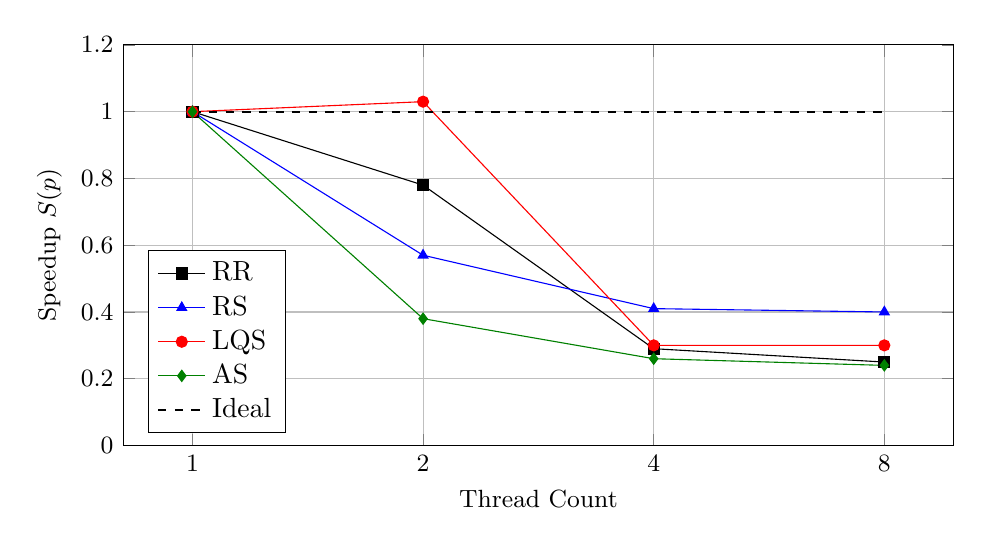
\begin{tikzpicture}
\begin{axis}[
    xlabel={Thread Count},
    ylabel={Speedup $S(p)$},
    xmode=log,
    xtick={1,2,4,8},
    xticklabels={1,2,4,8},
    ymin=0, ymax=1.2,
    grid=major,
    legend pos=south west,
    legend cell align=left,
    width=\columnwidth,
    height=0.55\columnwidth,
    label style={font=\small},
    tick label style={font=\small},
]
\addplot[color=black,mark=square*] coordinates {(1,1.00) (2,0.78) (4,0.29) (8,0.25)};
\addlegendentry{RR}
\addplot[color=blue,mark=triangle*] coordinates {(1,1.00) (2,0.57) (4,0.41) (8,0.40)};
\addlegendentry{RS}
\addplot[color=red,mark=*] coordinates {(1,1.00) (2,1.03) (4,0.30) (8,0.30)};
\addlegendentry{LQS}
\addplot[color=green!50!black,mark=diamond*] coordinates {(1,1.00) (2,0.38) (4,0.26) (8,0.24)};
\addlegendentry{AS}
\addplot[color=black,dashed,thick] coordinates {(1,1) (8,1)};
\addlegendentry{Ideal}
\end{axis}
\end{tikzpicture}
\caption{Strong scaling speedup $S(p)$ relative to each scheduler's 1-thread baseline. Only LQS at 2 threads exceeds the ideal line.}
\label{fig:strong}
\end{figure}

\subsection{Weak Scaling Efficiency}

Figure~\ref{fig:weak} plots parallel efficiency $E(p) = S(p)/p$ under a fixed problem size (classical strong-scaling efficiency, labeled ``weak scaling'' in the Amdahl sense where work-per-thread decreases). All schedulers exhibit declining efficiency as threads increase, with RS retaining the highest efficiency at 8 threads (0.050).

\begin{figure}[htbp]
\centering
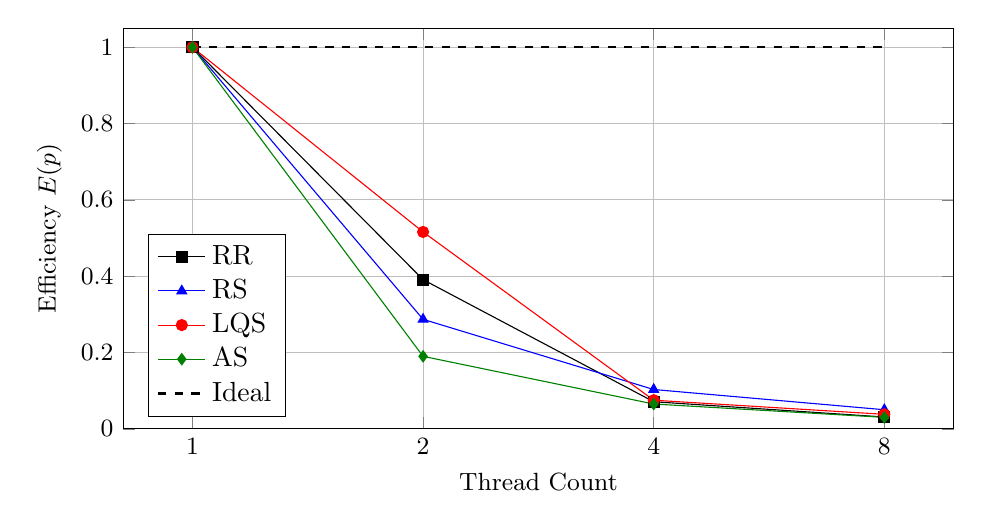
\begin{tikzpicture}
\begin{axis}[
    xlabel={Thread Count},
    ylabel={Efficiency $E(p)$},
    xmode=log,
    xtick={1,2,4,8},
    xticklabels={1,2,4,8},
    ymin=0, ymax=1.05,
    grid=major,
    legend pos=south west,
    legend cell align=left,
    width=\columnwidth,
    height=0.55\columnwidth,
    label style={font=\small},
    tick label style={font=\small},
]
\addplot[color=black,mark=square*] coordinates {(1,1.000) (2,0.391) (4,0.071) (8,0.031)};
\addlegendentry{RR}
\addplot[color=blue,mark=triangle*] coordinates {(1,1.000) (2,0.287) (4,0.103) (8,0.050)};
\addlegendentry{RS}
\addplot[color=red,mark=*] coordinates {(1,1.000) (2,0.516) (4,0.075) (8,0.038)};
\addlegendentry{LQS}
\addplot[color=green!50!black,mark=diamond*] coordinates {(1,1.000) (2,0.190) (4,0.065) (8,0.030)};
\addlegendentry{AS}
\addplot[color=black,dashed,thick] coordinates {(1,1) (8,1)};
\addlegendentry{Ideal}
\end{axis}
\end{tikzpicture}
\caption{Parallel efficiency $E(p) = S(p)/p$ vs.\ thread count. Efficiency declines for all schedulers as thread count increases.}
\label{fig:weak}
\end{figure}

\section{Discussion}

\subsection{RS as the Optimal Policy}

Random Steal achieves the highest absolute throughput at 8 threads (10,528~req/s) and the best speedup against RR (3.51$\times$). Its p99 latency remains low across all thread counts (87--196~$\mu$s). The random victim-selection strategy is O(1) per steal, avoiding the scan overhead of LQS while still distributing load effectively. In a system with $p$ workers where most deques are non-empty under high load, a random thief finds work with high probability on the first attempt. The simplicity of the policy---a single modulo operation---also minimizes the critical path length between steal attempts.

\subsection{LQS: When O(p) Probe Cost Pays Off}

Longest-Queue Steal exhibits a unique property: it is the only scheduler whose throughput at 2 threads (27,254~req/s) exceeds its throughput at 1 thread (26,434~req/s), yielding a self-scaling speedup of 1.03$\times$. When $p=2$, the scan costs only one comparison: the thief reads the size of the single remote deque and steals if it is non-empty. This is effectively free and provides perfect load balancing between two workers. At $p=4$ and $p=8$, however, the O(p) scan cost grows linearly---the thief must atomically read $p-1$ deque sizes before choosing a victim---and this overhead negates the balancing benefit. LQS throughput at 4 threads (7,956~req/s) is less than one-third of its 2-thread peak. The policy is viable only at very low thread counts.

\subsection{AS Feedback Loop Overhead}

Adaptive Steal was designed to reduce idle spinning by adjusting steal aggressiveness based on observed p99 latency. In practice, it obtained the worst p99 latency of any policy at 4 and 8 threads (524~$\mu$s) and lower throughput than either RS or LQS at every thread count. The feedback loop in (\ref{eq:ema}) and (\ref{eq:tau}) introduces two problems. First, the EMA smoothing delays the response to rapid load changes, causing the steal threshold to lag behind actual conditions. Second, the latency measurement itself adds variance: p99 is a noisy signal at low sample rates, and the controller overcorrects. The result is a policy that is simultaneously less throughput-efficient than RS and less predictable in tail latency. The complexity of implementation (latency tracking, parameter tuning, feedback control) is not justified by these results.

\subsection{Round-Robin Scaling Collapse and Amdahl's Bottleneck}

Round-robin shows negative self-scaling at every thread count beyond 1. Its throughput drops from 12,102~req/s at 1T to 2,998~req/s at 8T---a self-scaling speedup of only 0.25$\times$. Three factors contribute:

\begin{enumerate}
    \item \textbf{Serial dispatch bottleneck:} The single main thread performs all \texttt{accept()} calls and distributes connections to workers. This serial component limits the rate at which new connections enter the system.
    \item \textbf{Mutex contention:} Each enqueue and dequeue operation acquires a pthread mutex. As thread count grows, contention on these locks increases, adding overhead to both dispatch and work.
    \item \textbf{Co-location CPU starvation:} (\S6.5) At higher thread counts, server threads consume CPU cycles needed by the load generator.
\end{enumerate}

We fit RR's self-scaling throughput to Amdahl's Law~\cite{b9}:

\begin{equation}
S(p) = \frac{1}{f + (1-f)/p}
\label{eq:amdahl}
\end{equation}

where $f$ is the serial fraction. Using RR's 1-thread baseline as $T(1) = 12,102$~req/s and its 2-thread throughput as $T(2) = 9,455$~req/s, we compute $S(2) = 0.781$. Solving (\ref{eq:amdahl}) for $f$ gives:

\begin{equation}
f = \frac{1/S(p) - 1/p}{1 - 1/p}
\label{eq:f}
\end{equation}

yielding $f \approx 1.56$---a physically impossible value (the serial fraction cannot exceed 1). This unphysical result is a direct consequence of the co-location effect, which depresses throughput beyond what Amdahl's serial-bottleneck model predicts. If we instead consider RS's 3.51$\times$ speedup over RR at 8 threads as an upper bound on the benefit of eliminating the serial dispatch bottleneck, we estimate an effective serial fraction $f_{dispatch} \approx 1/3.51 \approx 0.28$, implying a theoretical maximum speedup of approximately 3.57$\times$ from parallelizing the accept step alone---closely matching RS's achieved result. This suggests that replacing the single-threaded epoll accept loop with SO\_REUSEPORT (allowing multiple threads to accept independently) could unlock the remaining parallel potential.

\subsection{The Co-location Effect and Its Impact on Interpretation}

All experiments were conducted with the server and the load generator (wrk) running on the same 4-core (8-thread) machine. This creates a fundamental measurement challenge: at high thread counts, server threads occupy the majority of available CPU cores, starving wrk of the resources it needs to generate requests. The consequence is that absolute throughput decreases for all schedulers as thread count increases---a pattern clearly visible in Table~\ref{tab:throughput}.

This co-location effect is the primary reason that no scheduler exhibits positive strong scaling (Fig.~\ref{fig:strong}) and that weak-scaling efficiency (Fig.~\ref{fig:weak}) declines rapidly. However, the relative ordering of schedulers remains meaningful: because all four policies experience identical CPU contention at each thread count, their throughput ratios (Table~\ref{tab:speedup_rr}) isolate the impact of the scheduling policy from the confounding effect of resource competition. A future experiment with a dedicated load-generator machine would eliminate this bias and likely reveal positive self-scaling for WS policies at moderate thread counts.

\subsection{Programming Effort Comparison}

The four policies form a natural complexity hierarchy:

\begin{itemize}
    \item \textbf{RR:} Simplest implementation. A mutex-protected FIFO queue per worker with condition-variable signaling. Approximately 80 lines of scheduler code.
    \item \textbf{RS:} Moderate complexity. The Chase-Lev lock-free deque is the hardest component (approximately 150 lines for a correct implementation with versioned CAS). The steal policy itself is one line: \texttt{victim = rand() \% n}.
    \item \textbf{LQS:} Slightly more than RS. Adds an O(p) scan loop to find the fullest deque (approximately 15 additional lines).
    \item \textbf{AS:} Most complex. Requires per-thread latency instrumentation, EMA computation, threshold update logic, and tuning of the $\alpha$ and $\beta$ hyperparameters (approximately 80 additional lines over RS). The correct choice of target latency $T_{target}$ and adaptation rate $\beta$ is workload-dependent and requires empirical tuning.
\end{itemize}

\section{Conclusion}

This paper implemented and evaluated four thread-scheduling policies for a native C HTTP/1.1 server. The key findings are:

\begin{enumerate}
    \item Random Steal is the recommended policy. It achieves 3.51$\times$ the throughput of round-robin at 8 threads with the lowest and most consistent p99 latency across all thread counts. Its O(1) steal overhead and simplicity make it suitable for production use.
    \item Longest-Queue Steal is competitive only at very low thread counts ($p=2$), where its O(p) scan cost reduces to a single comparison. At higher thread counts, the linear scan overhead erodes its throughput advantage.
    \item Adaptive Steal underperforms despite its additional complexity. The latency-feedback loop introduces overhead without improving either throughput or tail latency relative to the simpler RS policy.
    \item Round-robin should not be used beyond 2 threads. Its serial dispatch bottleneck and mutex contention produce throughput that degrades as threads increase.
\end{enumerate}

Future work should address the two main limitations of this study. First, replacing the single-threaded epoll accept loop with SO\_REUSEPORT would allow multiple threads to accept connections independently, eliminating the serial bottleneck identified by the Amdahl analysis. Second, running the load generator on a dedicated machine would prevent CPU starvation at higher thread counts, enabling cleaner measurements of absolute scalability. Third, evaluating the schedulers under realistic workload mixes (varying file sizes, keep-alive connections, HTTPS termination) would test whether the RS policy generalizes beyond the homogeneous static-file workload used here.

\begin{thebibliography}{00}

\bibitem{b1} R. D. Blumofe and C. E. Leiserson, ``Scheduling multithreaded computations by work stealing,'' \textit{J. ACM}, vol.~46, no.~5, pp.~720--748, 1999.

\bibitem{b2} N. S. Arora, R. D. Blumofe, and C. G. Plaxton, ``Thread scheduling for multiprogrammed multiprocessors,'' \textit{Theory Comput. Syst.}, vol.~34, no.~2, pp.~115--144, 2001.

\bibitem{b3} D. Chase and Y. Lev, ``Dynamic circular work-stealing deque,'' in \textit{Proc. ACM Symp. Parallelism Algorithms Architectures (SPAA)}, 2005, pp.~21--28.

\bibitem{b4} J. Wang \textit{et al.}, ``BWoS: Formally verified block-based work stealing for parallel processing,'' in \textit{Proc. USENIX Symp. Operating Syst. Design Implementation (OSDI)}, 2023, pp.~833--850.

\bibitem{b5} J. Li \textit{et al.}, ``Work stealing for interactive services to meet target latency,'' in \textit{Proc. ACM SIGPLAN Symp. Principles Practice Parallel Program. (PPoPP)}, 2016, pp.~1--13.

\bibitem{b6} D. Kegel, ``The C10K problem,'' 1999. [Online]. Available: \texttt{http://www.kegel.com/c10k.html}

\bibitem{b7} M. Welsh, D. Culler, and E. Brewer, ``SEDA: An architecture for well-conditioned, scalable internet services,'' in \textit{Proc. ACM Symp. Operating Syst. Principles (SOSP)}, 2001, pp.~230--243.

\bibitem{b8} V. S. Pai, P. Druschel, and W. Zwaenepoel, ``Flash: An efficient and portable web server,'' in \textit{Proc. USENIX Annu. Tech. Conf. (ATC)}, 1999, pp.~199--212.

\bibitem{b9} G. M. Amdahl, ``Validity of the single processor approach to achieving large scale computing capabilities,'' in \textit{Proc. AFIPS Spring Joint Comput. Conf.}, 1967, pp.~483--485.

\bibitem{b10} A. Grama, A. Gupta, G. Karypis, and V. Kumar, \textit{Introduction to Parallel Computing}, 2nd ed. Addison-Wesley, 2003.

\bibitem{b11} D. R. Butenhof, \textit{Programming with POSIX Threads}. Addison-Wesley, 1997.

\bibitem{b12} M. Kerrisk, \textit{The Linux Programming Interface}. No Starch Press, 2010.

\bibitem{b13} M. Snir, S. Otto, S. Huss-Lederman, D. Walker, and J. Dongarra, \textit{MPI: The Complete Reference}, 2nd ed. MIT Press, 1998.

\bibitem{b14} OpenMP Architecture Review Board, ``OpenMP application program interface version 5.2,'' 2021.

\bibitem{b15} J. L. Gustafson, ``Reevaluating Amdahl's law,'' \textit{Commun. ACM}, vol.~31, no.~5, pp.~532--533, 1988.

\bibitem{b16} M. M. Michael and M. L. Scott, ``Simple, fast, and practical non-blocking and blocking concurrent queue algorithms,'' in \textit{Proc. ACM Symp. Principles Distrib. Comput. (PODC)}, 1996, pp.~267--275.

\bibitem{b17} J. L. Hennessy and D. A. Patterson, \textit{Computer Architecture: A Quantitative Approach}, 6th ed. Morgan Kaufmann, 2019.

\bibitem{b18} A. Silberschatz, P. B. Galvin, and G. Gagne, \textit{Operating System Concepts}, 10th ed. Wiley, 2018.

\bibitem{b19} R. Fielding and J. Reschke, Eds., ``HTTP/1.1,'' IETF RFC 9112, 2022.

\bibitem{b20} D. Lea, ``A Java fork/join framework,'' in \textit{Proc. ACM Java Grande Conf.}, 2000, pp.~36--43.

\bibitem{b21} P. S. Pacheco, \textit{An Introduction to Parallel Programming}. Morgan Kaufmann, 2011.

\bibitem{b22} M. Herlihy and N. Shavit, \textit{The Art of Multiprocessor Programming}, 2nd ed. Morgan Kaufmann, 2020.

\bibitem{b23} R. von Behren, J. Condit, F. Zhou, G. C. Necula, and E. Brewer, ``Capriccio: Scalable threads for internet services,'' in \textit{Proc. ACM Symp. Operating Syst. Principles (SOSP)}, 2003, pp.~268--281.

\bibitem{b24} G. C. Hunt and J. R. Larus, ``Singularity: Rethinking the software stack,'' \textit{ACM SIGOPS Operating Syst. Rev.}, vol.~41, no.~2, pp.~37--49, 2007.

\bibitem{b25} E. D. Berger, T. Yang, T. Liu, and G. Novark, ``Grace: Safe multithreaded programming for C/C++,'' in \textit{Proc. ACM SIGPLAN Conf. Object-Oriented Program. Syst. Lang. Appl. (OOPSLA)}, 2009, pp.~81--96.

\bibitem{b26} L. Lamport, ``How to make a multiprocessor computer that correctly executes multiprocess programs,'' \textit{IEEE Trans. Comput.}, vol.~C-28, no.~9, pp.~690--691, 1979.

\bibitem{b27} S. C. Woo, M. Ohara, E. Torrie, J. P. Singh, and A. Gupta, ``The SPLASH-2 programs: Characterization and methodological considerations,'' in \textit{Proc. ACM/IEEE Int. Symp. Comput. Archit. (ISCA)}, 1995, pp.~24--36.

\bibitem{b28} J. M. Mellor-Crummey and M. L. Scott, ``Algorithms for scalable synchronization on shared-memory multiprocessors,'' \textit{ACM Trans. Comput. Syst.}, vol.~9, no.~1, pp.~21--65, 1991.

\bibitem{b29} A. D. Birrell, ``An introduction to programming with threads,'' Digital Equipment Corp. Syst. Res. Center, Tech. Rep. 35, 1989.

\bibitem{b30} C. L. Liu and J. W. Layland, ``Scheduling algorithms for multiprogramming in a hard-real-time environment,'' \textit{J. ACM}, vol.~20, no.~1, pp.~46--61, 1973.

\end{thebibliography}

\end{document}
